\documentclass[12pt, letterpaper]{article}
\usepackage{amsmath,amssymb}
\usepackage{graphicx,float}
\usepackage{hevea}
\usepackage{hyperref,hypcap}
\begin{document}

\title{Super Four Bar Explorer Professional Deluxe Edition 2008-X: A Spiritual Journey on Solving the Reverse Kinematics Problem for a General Four-Bar Linkage using a Least Orthogonal Squares Curve Fit Algorithm}
\author{Joshua Holbrook}
\date{\today}
\maketitle

%\section*{The Problem}

``What's the point?'' I asked myself.  It's also, in a moment of brashness, what I asked Dr. Lin.

We'd been discussing how to calculate the velocities and accelerations involved in a specific four-bar linkage in a specific position, using the graphics method.  What bothered me about it was that, for all this work, all one could ascertain was an instantaneous velocity and acceleration at only one of an infinite amount of positions for a linkage. Moreover, in most cases one doesn't have a linkage already designed---instead, he has a set of requirements that the linkage has to meet---passing through certain positions at certain speeds or accelerations.

I don't remember exactly what he said. He talked about how synthesis is a tough problem, and mentioned off-hand a few approaches to take, and a few software packages we could use. I'd allowed myself to be momentarily distracted when I heard him say something along the lines of ``curve fitting.'' This got my attention. Curve fits are optimization problems, something I'd seen before.

My plan became to create a program that could fit a linkage to a set of points that one wanted a traced path to travel through, given a starting linkage. If this was successful, the algorithm could be adapted to take velocity, acceleration, or transmission angle into account. I would consider the algorithm a partial success if I could get it to work in particularly ``nice'' situations, and a strong success if I could get it to work for a wider range of situations, where complications would come into play.

Ostensibly, this program is similar to Lincages, as seen in figure \ref{fig:lincages} .

\begin{figure}[H]
\centering
\caption{Arguably, My Program's Already Better Than This.}
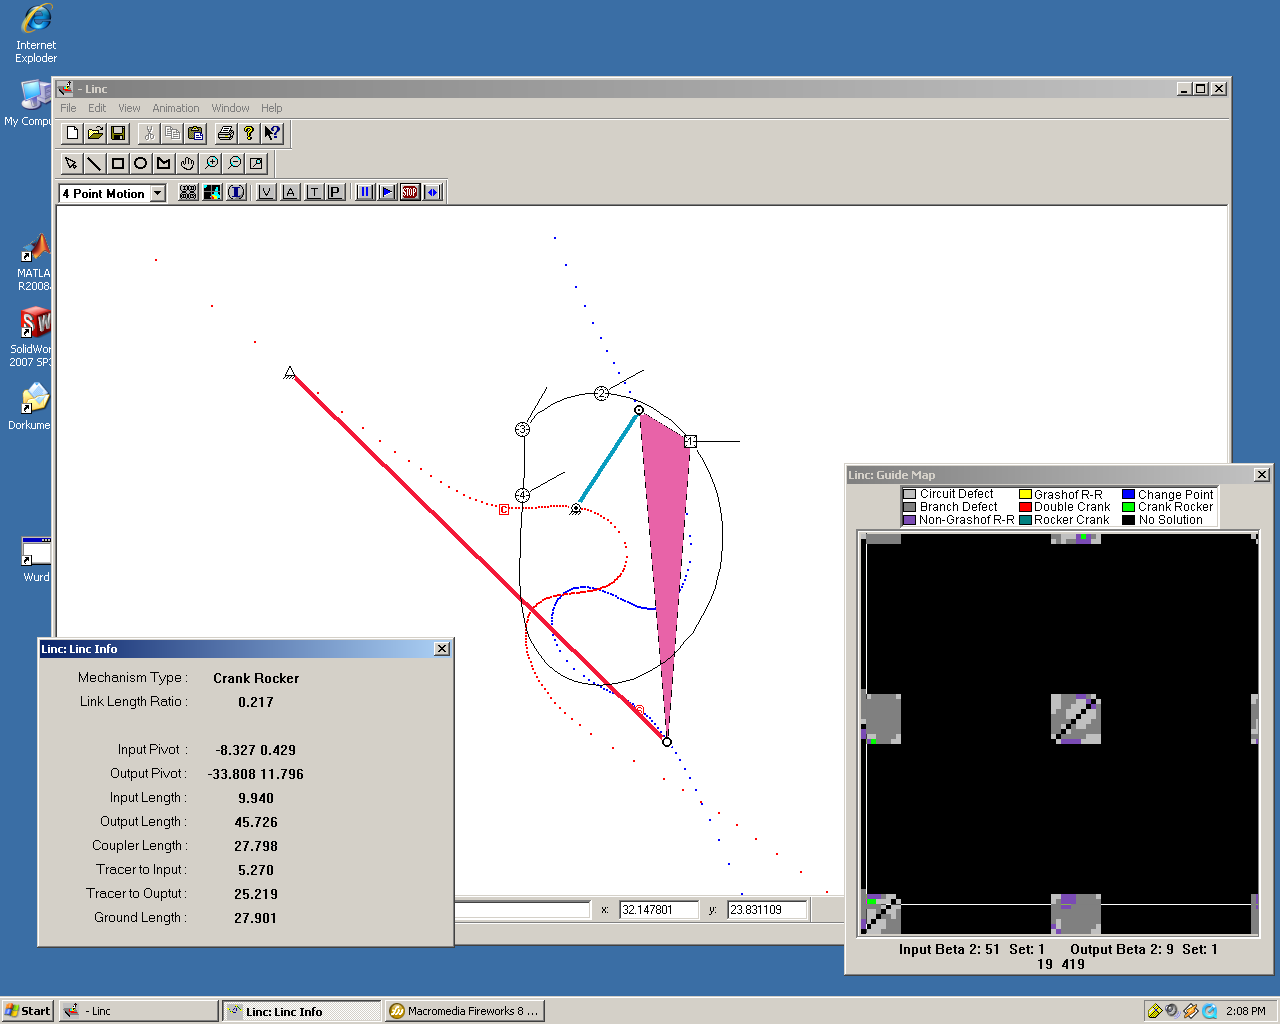
\includegraphics[width=4.5in]{lincages}
\label{fig:lincages}
\end{figure}

Lincages takes a different approach to this problem (as I'll address later) and is much more feature-rich (though severely lacking in polish---as an aside, I think the Lincages people should be ashamed to be selling their software commercially), but the general idea of designing a linkage to pass through a set of points is the same between them.

\section*{Forward Kinematics}

A good starting place for this problem is figuring out the analytical equation(s) for the path traced by a given four-bar linkage.

\begin{figure}[H]
\centering
\caption{My Calligraphy Skills are Unparalleled.}
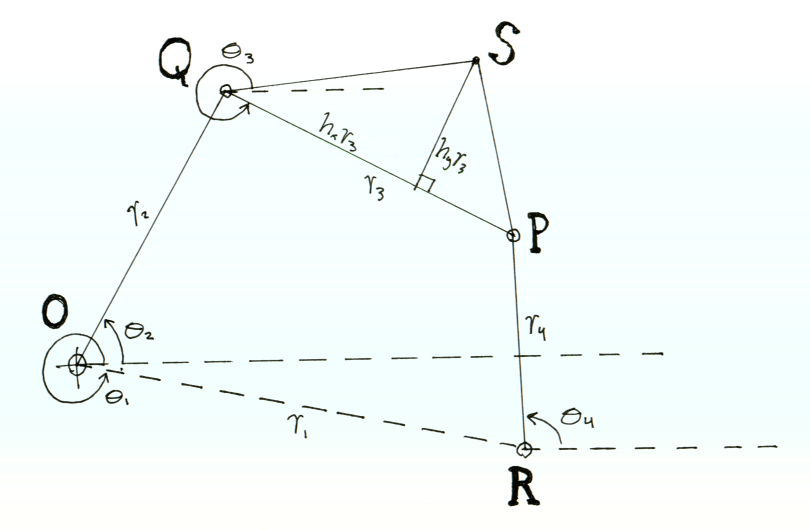
\includegraphics[width=4.0in]{fourbar}
\label{fig:fourbar}
\end{figure}

The equations in this section come from section 5.3 of ``Kinematics, Dynamics, and Design of Machinery,'' Second Edition, by Kenneth J. Waldron and Gary L. Kinzel, as are most of the choices of symbol (\(h\), \(S\) and \(\tilde{S}\) being exceptions).

The basis for all the equations used for the four-bar linkage comes from the fact that four bars form a closed loop. As a result, if each member is represented as a vector, then:
\[r_2\begin{pmatrix}\cos\theta_2 \\ \sin\theta_2\end{pmatrix}+
r_3\begin{pmatrix}\cos\theta_3 \\ \sin\theta_3\end{pmatrix}=
r_1\begin{pmatrix}\cos\theta_1 \\ \sin\theta_1\end{pmatrix}+
r_4\begin{pmatrix}\cos\theta_4 \\ \sin\theta_4\end{pmatrix}\]

In my specific case, \(r_1\) is the ground link (meaning its angle is a constant), and \(r_2\) is the driver link.

By using a number of trigonometric ratios to eliminate \(\theta_3\) and formulate a quadratic equation problem,  these equations can be solved for \(\theta_4\) given all the \(r_i\) and \(\theta_1\) and \(\theta_2\):

\[\theta_4=2\tan^{-1}\left(\frac{-B+\sigma\sqrt{B^2+C^2-A^2}}{C-A}\right)\]
where
\begin{align*}
A&=2r_1r_4\cos\theta_1-2r_2r_4\cos\theta_2\\
B&=2r_1r_4\sin\theta_1-2r_2r_4\sin\theta_2\\
C&=r_1^2+r_2^2+r_4^2-r_3^2-2r_1r_2\left(\cos\theta_1\cos\theta_2+\sin\theta_1\sin\theta_1\right)\\
\sigma&=\pm1
\end{align*}

\(\sigma\) is a parameter used to pick the proper configuration of the linkage, since there are two of them that solve this system.

\begin{figure}[H]
\centering
\caption{``Whoa! There's two of them!'' --Strong Bad}
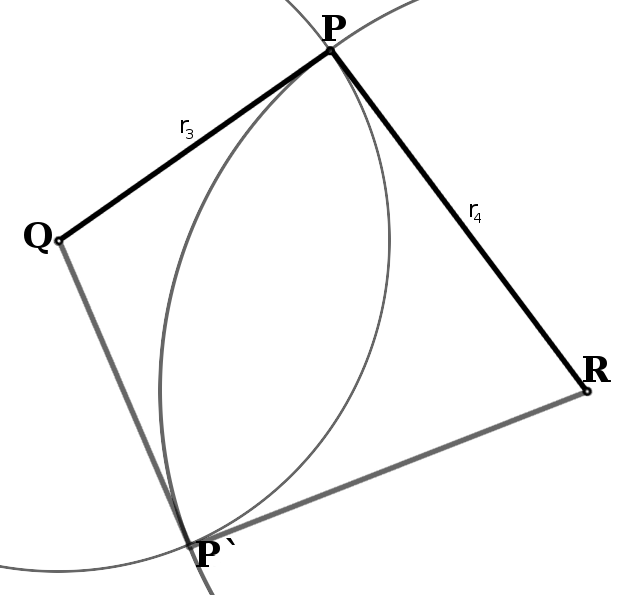
\includegraphics[width=2.5in]{dyad}
\label{fig:dyad}
\end{figure}

Note that there is a square root which may potentially be imaginary.  This would mean that the linkage can't be physically assembled in that configuration---in most cases, this would simply mean that \(\theta_2\) is outside the allowable range for that linkage, though there are also certainly cases where the linkage can't be assembled at all.

Anyways---With \(\theta_4\), finding the position \(P\) is simple enough:

\[P=O+r_1\begin{pmatrix}\cos\theta_1\\ \sin\theta_1\end{pmatrix}+
r_4\begin{pmatrix}\cos\theta_4\\ \sin\theta_4\end{pmatrix}\]

Note: \(O\) is the position of the origin. Usually this is set to \(0,0\), but I would like to allow this to change in my function.

Of course, the position \(Q\) was always easy to find:

\[Q=O+r_2\begin{pmatrix}\cos\theta_2\\ \sin\theta_2\end{pmatrix}\]

I decided to define the tracing point \(S\) using \(P-Q\) and \(R_{90^0}\left(P-Q\right)\) as a basis, where \(R_{90^0}\) is a \(90^0\) rotation matrix:

\[S=\begin{bmatrix}
\uparrow & \uparrow\\
P-Q & R_{90^0}\left(P-Q\right)\\
\downarrow & \downarrow
\end{bmatrix}
h
+Q\]

where the vector \(h\) controls the position of \(S\) relative to \(P-Q\).

Alternately, this form that will be more convenient at a later date:

\[\begin{pmatrix}S_x\\S_y\end{pmatrix}=
\begin{pmatrix}(1-h_x)Q_x+h_xP_x+h_y\left(Q_y-P_y\right)\\
(1-h_x)Q_y+h_xP_y+h_y\left(P_x-Q_x\right)\end{pmatrix}\]

I programmed these equations into Gnumeric (a spreadsheet program much like Microsoft Excel) in order to not only test my forward equations, but also to test various parameters to get a more intuitive feel on how linkages behaved as I changed parameters, to generate test points for the curve fit algorithm, and to eventually test the results of said algorithm. Figure \ref{fig:plotter} shows a screenshot of this ''software."

\begin{figure}[H]
\centering
\caption{Computer Science Majors Fear Me.}
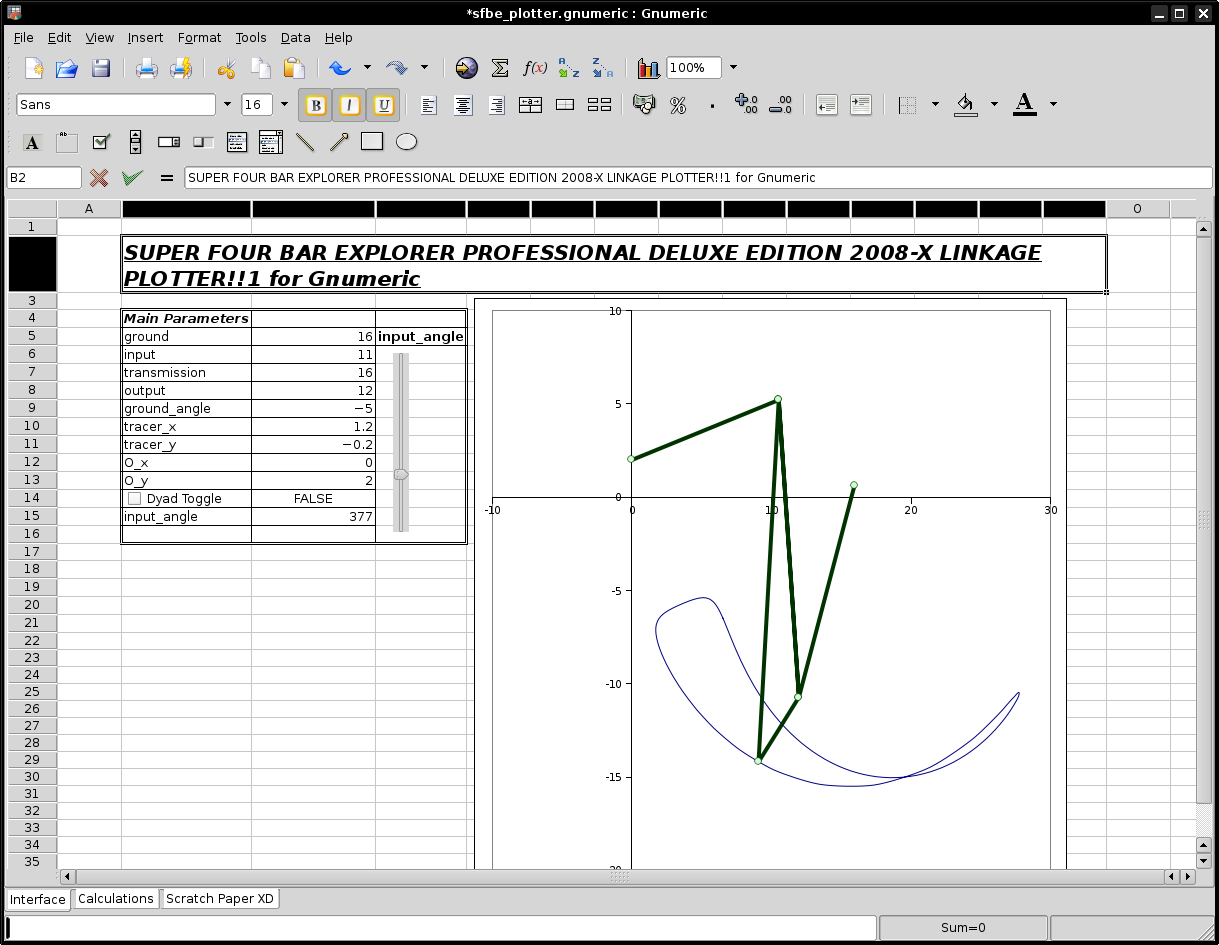
\includegraphics[width=5.0in]{plotter}
\label{fig:plotter}
\end{figure}

Perhaps worth noting is that a spreadsheet is perhaps the least elegant method I could've used to encode these equations (I would argue that TI Basic would be worse). As a programmer friend of mine says, ``spreadsheets are full of fail.'' On the plus side, spreadsheets typically have excellent graphing tools, and Gnumeric is no exception to this rule. It was this, combined with my laziness and my high levels of familiarity with spreadsheets (I do have an engineering background after all) that led to my choice of ``development platform." As an added bonus, a graphical user interface for changing the parameters was included whether I wanted it or not.

\section*{Reverse Kinematics}

Going backwards is, of course, another matter entirely. The problem basically comes down to a system of the forward equations with fixed \(\tilde{S}_x\) and \(\tilde{S}_y\) that have to be solved for all the \(r_i\) and \(\theta_1\).

There are a number of approaches to this. In fact, these approaches generalize to pretty much any linkage.

One basic and time-tested approach is simple trial-and-error: That is, design a linkage, look at what the path does, and change the parameters, by hand, in a somewhat intelligent manner, until the linkage fits the design criteria. While this approach is still taught, I would like to think that, with today's technology, there is a better way.

For what might be considered a more sensible approach, these equations can be reformulated as quadratic equations quite simply by substituting \(\sin\theta_i\) and \(\cos\theta_i\) with variables--say, \(s_i\) and \(c_i\) respectively--and constraining them to satisfy the identity \(\sin^2\theta + \cos^2\theta = 1\). Then, if one knows what he is doing, they can be solved analytically using a process similar to Gaussian elimination but more general (called, according to Wikipedia, Buchberger's algorithm). Naturally, \emph{I} don't know what I'm doing, but that won't stop me from commenting on it anyway. Another technique used to simplify the equations is to invoke Euler's formula (\(e^{i\theta}=\cos\theta + i\sin\theta\)) and solve \(r_2e^{i\theta_2}+r_3e^{i\theta_3}=r_1e^{i\theta_1}+r_4e^{i\theta_4}\). I can't claim to know for sure, but it is my impression that it is this method that this is the method that Lincages uses.

An obvious advantage to analytical methods is that any solution(s) will be exact analytical ones.  This is especially nice if there are multiple linkages that satisfy the system of equations, since it will result in an equation that describes all the solutions to the equation.

There are also other numerical methods that can be used to solve this problem. For example, the CUIK Project (\url{http://www-iri.upc.es/groups/cinemat/cuikweb/}) uses a series of techniques it calls ``box shrinking'' and ``box splitting'' to approximate solutions for generalized position analysis problems.

The approach I take---that is, solving a curve fitting problem---does have advantages over, at least, analytical solutions; If there is no analytical solution, then the process will still yield a ''least squares solution," which, while not technically a solution, is by some measure the closest thing to an exact solution. It also has the advantage of being something I'm already relatively familiar with. On the other hand, it's not an approach that seems to be in wide use, which suggests (to me) that it may not behave very well in practice.

\section*{The Objective Function}

The overwhelmingly-used reference for this section was ``Numerical Optimization'', Second Edition, by Jorge Nocedal and Stephen J. Wright.

Given a set of points of the form \((x_j,y_j)^T\) to fit the curve to, a vector \(v\) containing \(r_1,r_2,r_3,r_4,\theta_1,h_x,h_y,O_x\) and \(O_y\), and a vector \(\vec{\theta}\) containing all the \((\theta_2)_j\) for each point, the problem I want to solve (again, initially) is the following:

\[\min_{v,\vec{\theta}}\sum_{j=1}^m\left|\left|\begin{pmatrix}\tilde{S}_x(v,\vec{\theta}_j)\\ \tilde{S}_y(v,\vec{\theta}_j)\end{pmatrix}-\begin{pmatrix}x_j\\y_j\end{pmatrix}\right|\right|\]

or, alternately:

\[\min_{v,\vec{\theta}}\sum_{j=1}^{2m}r_j^2\]
where
\[r_j=\left\{\begin{array}{l l}
(\tilde{S_x})_j(v,\vec{\theta}_j)-x_j & \text{ for } j \in [1,m]\\
(\tilde{S_y})_{j-m}(v,\vec{\theta}_{j-m})-y_{j-m} & \text{ for } j \in [m+1,2m]\end{array}\right.\]

\(r_j\) is known as the jth residual.

Unfortunately, there's a clash here amongst conventions.  \(r_i\) is used in kinematics to refer to the length of the ith member of a linkage, while \(r_j\) is used to refer to the jth residual in the formulation of a least squares problem.It's currently not very important, but it may be cause for confusion in the future.

Note that, unlike in many curve fitting applications, the variable \(\theta_j\) is merely a parameter whose value is allowed to change, since I'm only really interested in how \(\tilde{S}_x\) and \(\tilde{S}_y\) relate to each other.

The prototypical unconstrained optimization solution-finding technique is an iterative process:
\[x_{k+1}=x_k+\alpha_kp_k\]
\(x_k\) represents a point---in my case, it's a set of parameters describing the four-bar linkage.  \(p_k\) represents a search direction, and \(\alpha_k\) is a scaling factor, called a ``step size.'' Often, a line search technique is used, where a search direction is chosen first, and then an appropriate \(\alpha_k\) is figured out. A very common technique, and one the reader is likely at least passably familiar with, is Newton's Method. 

Since this is a variation of a least squares curve fit problem, I should be able to use the Gauss-Newton Method to solve it, where the direction is chosen by solving the following matrix equation:

\[J^TJp_{k}=-J^T\vec{r}\]

where \(p_k\) is (again) a search direction, \(J\) is the Jacobian of \(\vec{r}\), and \(\vec{r}\) contains all the residuals \(r_j\).

The Gauss-Newton Method is an approximation of Newton's Method (and as such is in the family of ``Quasi-Newton Methods'') that uses \(\vec{r}\) and the Jacobian of \(\vec{r}\) instead of the Hessian and the gradient of the objective function, respectively, in finding \(p_k\). For problems of this form, \(J^TJ\) well-approximates the Hessian (for well-posed problems, anyway) and \(J^T\vec{r}\) is exactly the gradient of the objective function.

\section*{The Jacobian}

Perhaps the toughests part of this project involve calculating the Jacobian required for the Gauss-Newton Method.

As previously mentioned, this problem is different from many curve fitting problems in that the input parameter, \((\theta_2)_j\), doesn't matter to me and as such is allowed to change. Aside from making me unsure about the performance of this method for this case, it meant I had to think about what the Jacobian of the function would look like.

A Jacobian, in general, looks like this:

\[J_x(\vec{r})=\begin{pmatrix}
\leftarrow & \bigtriangledown_xr_1 & \rightarrow \\
\leftarrow & \bigtriangledown_xr_2 & \rightarrow \\
& \vdots & \\
\leftarrow & \bigtriangledown_xr_m & \rightarrow
\end{pmatrix}\]

where x is all the input variables for the function, and n is the number of residuals in the objective function (in this case, \(2m\)).

In this case, though, each residual \(r_j\) involves \(\theta_j\). After much thought, I had an epiphany of what probably should've been obvious:

\[\text{Let } v=\begin{pmatrix}r_1\\r_2\\r_3\\r_4\\\theta_1\\h_x\\h_y\\O_x\\O_y\end{pmatrix} \text{ and } \vec{\theta}=\begin{pmatrix}(\theta_2)_1 \\ (\theta_2)_2 \\ \vdots \\ (\theta_2)_m\end{pmatrix}\]

\[J=\begin{pmatrix}
\leftarrow & \bigtriangledown_vr_1 & \rightarrow & \frac{\partial r_1}{\partial(\theta_2)_1} & 0 & \dots & 0\\
\leftarrow & \bigtriangledown_vr_2 & \rightarrow & 0 & \frac{\partial r_2}{\partial(\theta_2)_2} & \dots & 0\\
\leftarrow & \vdots & \rightarrow & \vdots & \vdots & \ddots & \vdots\\
\leftarrow & \bigtriangledown_vr_m & \rightarrow & 0 & 0 & \dots & \frac{\partial r_m}{\partial(\theta_2)_m}\\
\leftarrow & \bigtriangledown_vr_{m+1} & \rightarrow& \frac{\partial r_{m+1}}{\partial (\theta_2)_{m+1}} & 0 & \dots & 0\\
\leftarrow & \vdots & \rightarrow & 0 & \frac{\partial r_{m+2}}{\partial (\theta_2)_{m+2}} & \dots & 0\\
\leftarrow & \vdots & \rightarrow & \vdots & \vdots & \ddots & \vdots\\
\leftarrow & \bigtriangledown_vr_{2m} & \rightarrow & 0 & 0 & \dots & \frac{\partial r_{2m}}{\partial(\theta_2)_{2m}}
\end{pmatrix}\]

It looks ugly, but that has more to do with my sense of aesthetics than it does with the actual meaning of the thing. Basically, all I'm saying is that all the gradients of the residuals are with respect to \((v^T \; | \; \vec{\theta}^T)^T\), and that this results in a block form for \(J\) with two diagonal matrices and a typical, pedestrian Jacobian with respect to \(v\).

Finally, since \(r_j=(\tilde{S}_x)_j-x_j\) for \(j \in [1,m]\) and \((\tilde{S}_y)_{j-m}-y_{j-m}\) for \(j \in [m+1,2m]\), and \(x_j\) and \(y_{j-m}\) are all constant terms, \(r_j\) can safely be replaced by \((\tilde{S}_x)_j\) and \((\tilde{S}_y)_{j-m}\) as appropriate.

\[J=\begin{pmatrix}J_x & D_x \\ J_y & D_y\end{pmatrix}\]
where
\[\begin{matrix}J_x=\begin{pmatrix}
\leftarrow & \bigtriangledown_v(\tilde{S}_x)_1 & \rightarrow\\
\leftarrow & \bigtriangledown_v(\tilde{S}_x)_2 & \rightarrow\\
& \vdots &\\
\leftarrow & \bigtriangledown_v(\tilde{S}_x)_m & \rightarrow
\end{pmatrix}
&
J_y=\begin{pmatrix}
\leftarrow & \bigtriangledown_v(\tilde{S}_y)_1 & \rightarrow\\
\leftarrow & \bigtriangledown_v(\tilde{S}_y)_2 & \rightarrow\\
& \vdots &\\
\leftarrow & \bigtriangledown_v(\tilde{S}_y)_m & \rightarrow
\end{pmatrix}
\end{matrix}\]
\[\begin{matrix}
(D_x)_{i,j}=\left\{\begin{array}{l l}
\frac{\partial\tilde{S}_x}{\partial\vec{\theta}_i} & \text{ for } i=j\\
0 & \text{ for } i \ne j
\end{array}\right.
&
(D_y)_{i,j}=\left\{\begin{array}{l l}
\frac{\partial\tilde{S}_y}{\partial\vec{\theta}_i} & \text{ for } i=j\\
0 & \text{ for } i \ne j
\end{array}\right.
\end{matrix}\]

A final point:  I chose to use a technique called ``backtracking'' to choose the step size \(\alpha\), in which I start with an initial alpha and keep multiplying it by a number between zero and one until it yields a sufficiently better fit. This is defined properly both in my program and on page 37 of Nocedal and Wright, but the details aren't at all ground-breaking or interesting.  I chose backtracking because it's simple and because I've implemented it before and as such have some level of familiarity with the technique.

\section*{Going For It: Programming the First Prototype}

The programming of the prototype went through a number of distinct phases.

In the first phase, I found all the necessary derivatives of \(\tilde{S}_x\) and \(\tilde{S}_y\) using SymPy, a CAS library for python. I decided to use SymPy because I already had it installed on my computer and because I'm already somewhat familiar with python.  The position equations are quite nasty (something that is partially obscured by the modularization of the equation), so the derivatives were, perhaps predicatably, also very nasty. In fact, they were pages long and not very enlightening to look at. Despite this, I did put the effort into getting them formatted in \LaTeX, and put them into an html file using \hevea, a \LaTeX to html converter. For the record, I did attempt to run a simplification algorithm on them, but gave up on it after it ``spun its wheels'' for an hour or so without making headway. Once I had these equations, I pasted them into my code.

As an aside: Something I find disappointing is that I can no longer get a feel as to whether the solution(s) might be correct by intuition because of the lengths of the expressions. Basically, I had to hope that SymPy isn't letting me down.

I chose to use Python for the main program as well, with SciPy, a numerical library. I had originally talked about using Haskell for this task, a functional language that lends itself very well to describing mathematics. Unfortunately, I knew Python but not Haskell, and deadlines forced me to choose the one I was more familiar with at the risk of a loss of elegance.

After getting rid of the initial bugs in this first version of the program and running it against a test case, I kept getting "NaN" feedback from various calculations within the program. This was somewhat alarming, and since I couldn't properly debug the program with those massive cryptic expressions.

So, the second phase involved me trying to incorporate SymPy's symbolic differentiation abilities into the program, but this caused a whole new mess of problems.  After a bunch of work, I decided that it was possible (even likely) that it was a problem with SymPy. SymPy is still in development, and this becomes clear as one begins to use it through its lack of polish and contradicting documentation. A caveat, however: I'm fairly unskilled as a programmer, so it is possible, even likely, that I was the one screwing up yet blaming SymPy for my problems.

The third phase began when I decided to look into SciPy's abilities to take numerical derivatives. It turns out that SciPy has a nice function for doing so, but it only works on functions of one variable. I got around this by using lambdas, also known as anonymous functions. For an example:

\begin{verbatim}
derivative(lambda a: Sx(a,r2,r3,r4,t1,hx,hy,Ox,Oy,sig,t2),r1,0.01*r1)
\end{verbatim}

Many would call this a kludge, but I'm honestly fairly proud of myself for figuring this one out.

Also demonstrated in this is one of the many problems I found while debugging during this phase, which is that the standard \(dx\) for SciPy's derivative function is 1, which for some problems at least was quite large---large enough, in fact, to ``break'' my algorithm by trying to take sample points outside the domain of the position function.

I then spent a long time debugging the program, finding some interesting problems (such as the one I just explained) and some dumb problems (such as finding significant typographical errors in my forward equations). Finally, after much work, I was able to get a ``close'' example to generate a plausible solution. After three days of coding and debugging, I finally had success.

At this point, I made a change to the backtracking code to deal with the fact that the initial step size may not only fail to yield sufficient decrease, but may also take \(x_{k+1}\) outside the feasible region. This improved the stability of the algorithm significantly.

\section*{Benchmarking}

I chose a first problem to demonstrate that the algorithm would work for a ``nice'' example. I did this by constructing a linkage with my gnumeric spreadsheet, using a randomized function to generate a set of points somewhat close and normally distributed around the curve (with \(\sigma=0.3\)), and running those numbers along with the linkage parameters used as a starting point, inside my program.  If the program was to work, then it should converge reasonably quickly to a solution near the starting point.

Though the first prototype has some problems, it seemed to work quite well. Compare figure \ref{fig:initial_problem}, depicting the input parameters against the points to fit, and figure \ref{fig:initial_solution}, depicting the output parameters against the points to which they were chosen to fit:

\begin{figure}[H]
\centering
\caption{The Initial Problem}
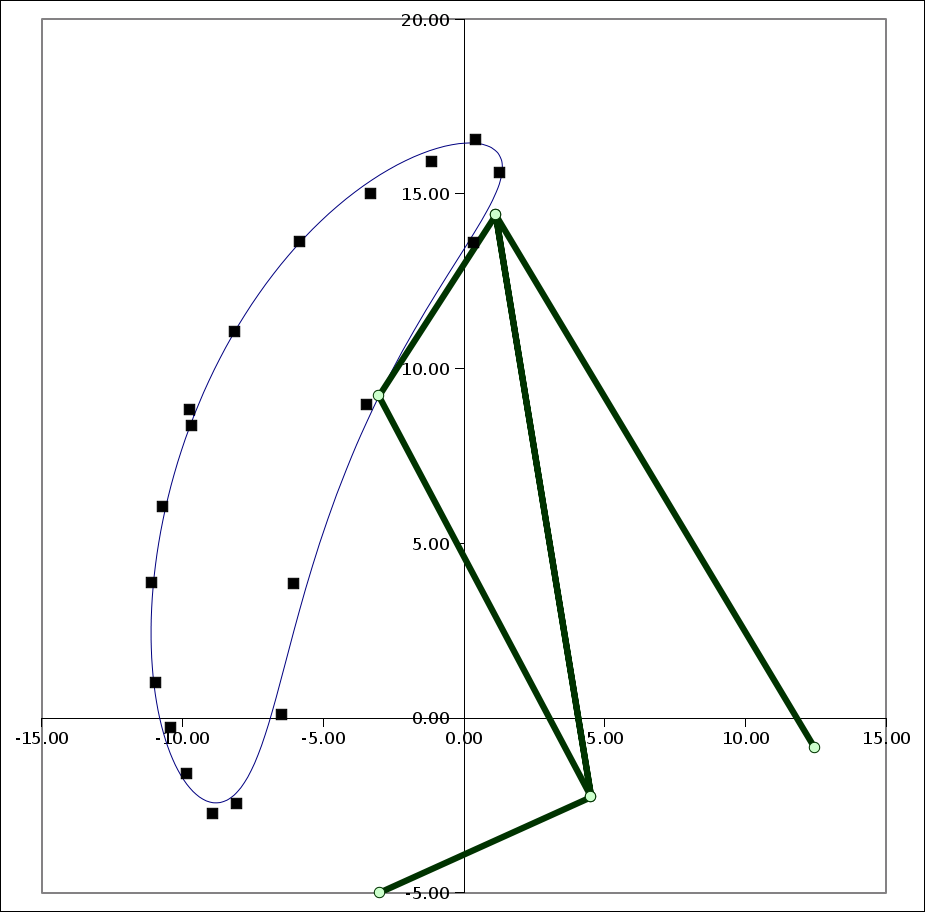
\includegraphics[width=3.0in]{initial_problem}
\label{fig:initial_problem}
\end{figure}

\begin{figure}[H]
\centering
\caption{The Initial Solution}
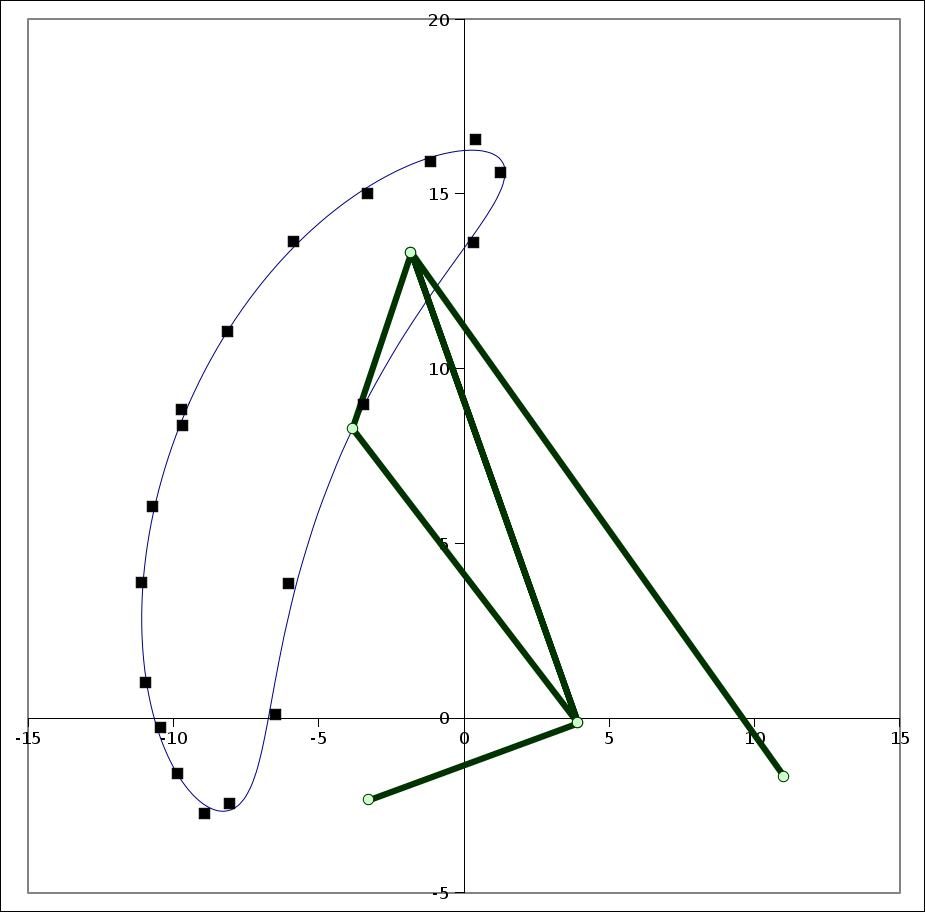
\includegraphics[width=3.0in]{initial_solution}
\label{fig:initial_solution}
\end{figure}

Graphically, this lends plausibility to the solution, but it's tough to see if the second is an improvement by visual inspection alone. However, checking the sums of the residuals in the output of the program puts this issue to rest:

\begin{verbatim}
josh@gengar:~/College 2008-2009/sfbe$ ./promblem.py
The output of sfbe.linkagefit for the "close" problem is:

r_1:  14.2682589754
r_2:  7.53613267311
r_3:  14.6801053812
r_4:  19.6737879912
t_1:  0.0539836197056
h_x:  0.737880586557
h_y:  0.262858101874
O_x:  -3.25616992596
O_y:  -2.39564861511

The sum of the squares of the original residuals was:  2.21532300525

The sum of the squares of the new residuals is:  0.458750196675
\end{verbatim}

Clearly, this was an improvement.

Then, I tried the problem again, but with a less-than-ideal starting point:

\begin{figure}[H]
\centering
\caption{A Somewhat More Difficult Starting Point}
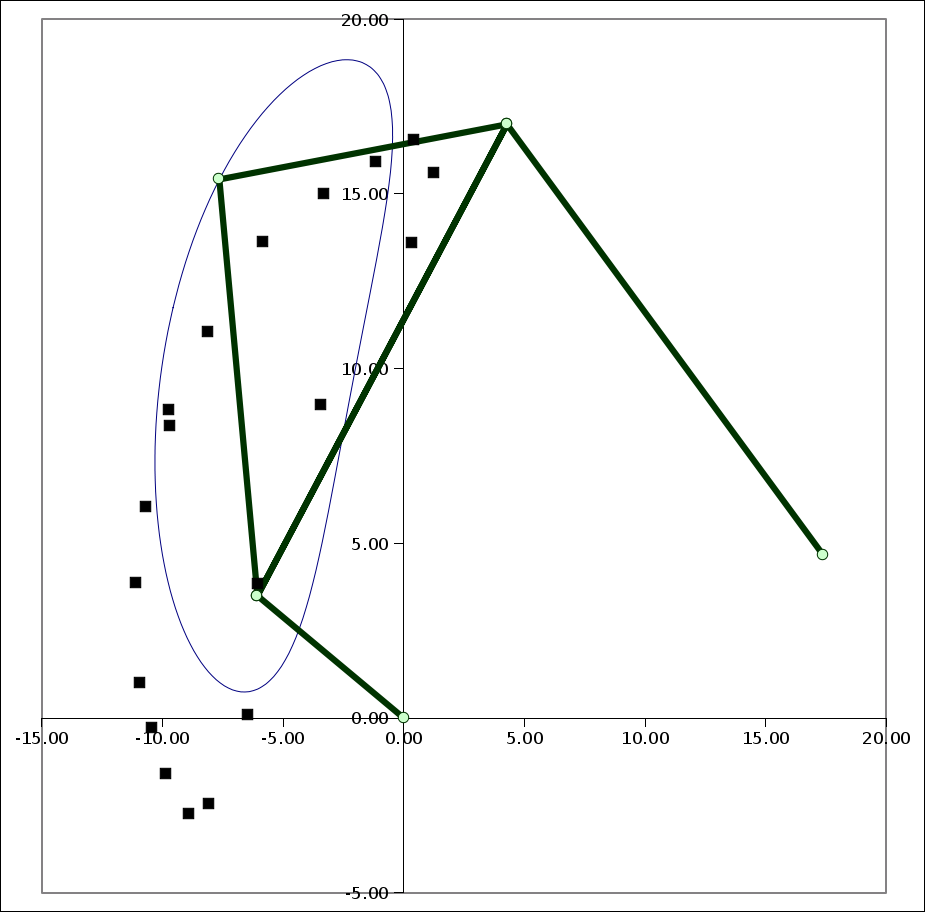
\includegraphics[width=3.0in]{medium_problem}
\label{fig:medium_problem}
\end{figure}

\begin{figure}[H]
\centering
\caption{The Algorithm Still Converges}
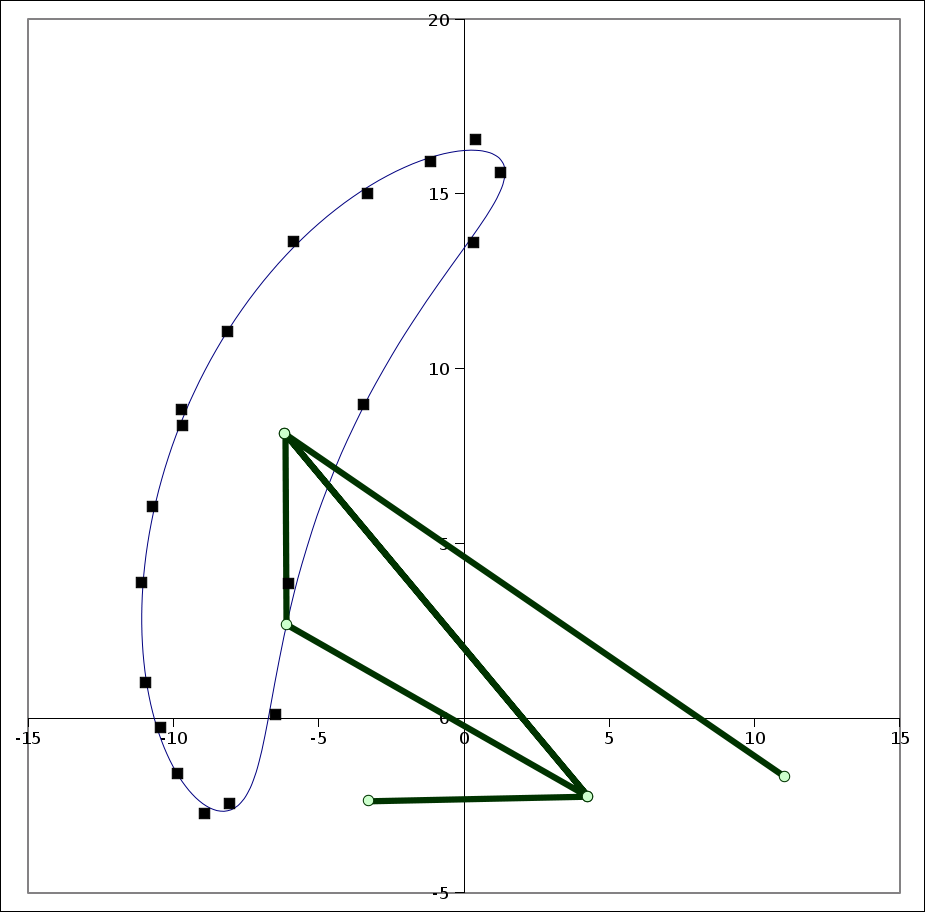
\includegraphics[width=3.0in]{medium_solution}
\label{fig:medium_solution}
\end{figure}

And, for hard numbers:
\begin{verbatim}
The sum of the squares of the original residuals was:  214.828696028

The sum of the squares of the new residuals is:  0.458624516185
\end{verbatim}

In this case, one can see significant improvement of the linkage, given the design criteria.

However, as I found out, the algorithm does rely on having a decent starting point.  I tried a much worse starting point, as illustrated in figure \ref{fig:bad_problem}, and with it the algorithm did not converge.

\begin{figure}[H]
\centering
\caption{I Don't Think I Ask For Too Much, Do You?}
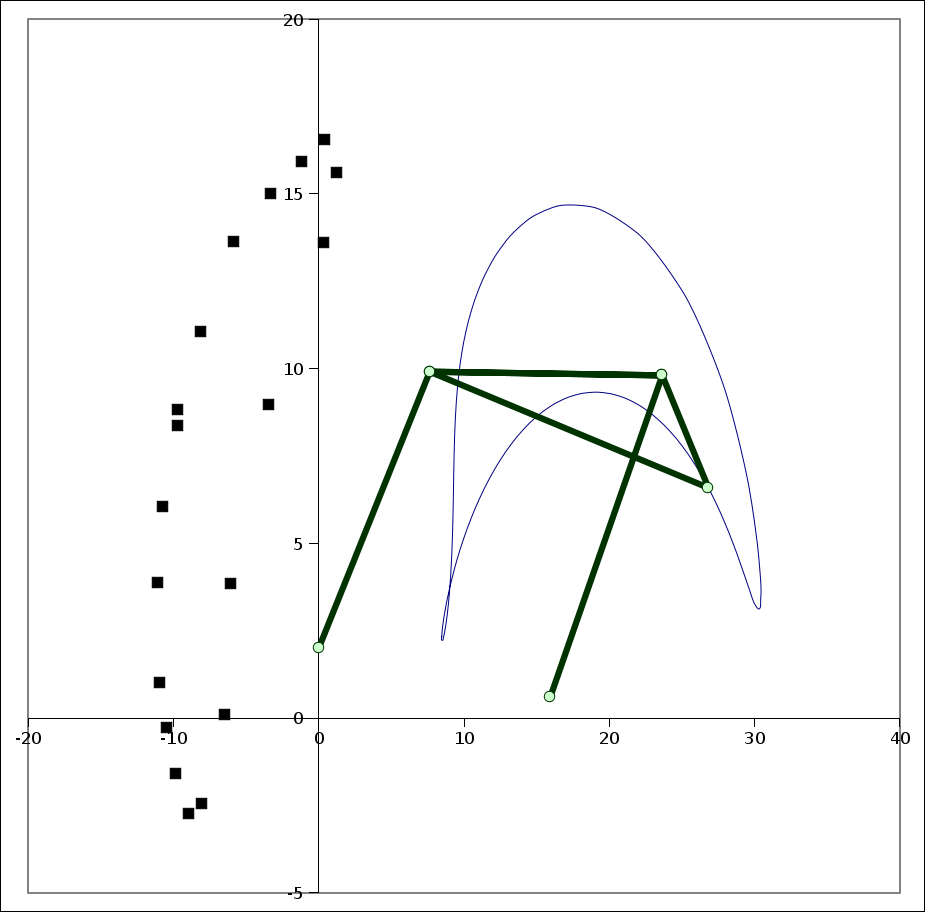
\includegraphics[width=3.0in]{bad_problem}
\label{fig:bad_problem}
\end{figure}

Finally, I attempted to come up with a plausible example of how this could be used to design an actual linkage. Suppose I wanted to create a linkage that travels through the data points in table \ref{tab:datapoints}.

\begin{table}[H]
    \centering
    \caption{I Like My Linkages The Way I Like My Whiskey.}
    \begin{tabular}{r l}
    x & y \\ \hline
    0 & 0\\
    2 & 2\\
    4 & 4\\
    6 & 6\\
    8 & 8\\
    10 & 10
    \end{tabular}
    \label{tab:datapoints}
\end{table}

In words, I would like my linkage to travel in a straight line.

I started by using the linkage plotting spreadsheet to find a somewhat close starting point without particularly straining myself, as seen in Figure \ref{fig:apply_problem}, Table \ref{tab:startingv} and Table \ref{tab:startingthetas}.

\begin{figure}[H]
\centering
\caption{Man, Using This Software is \emph{So} \emph{Hard}}
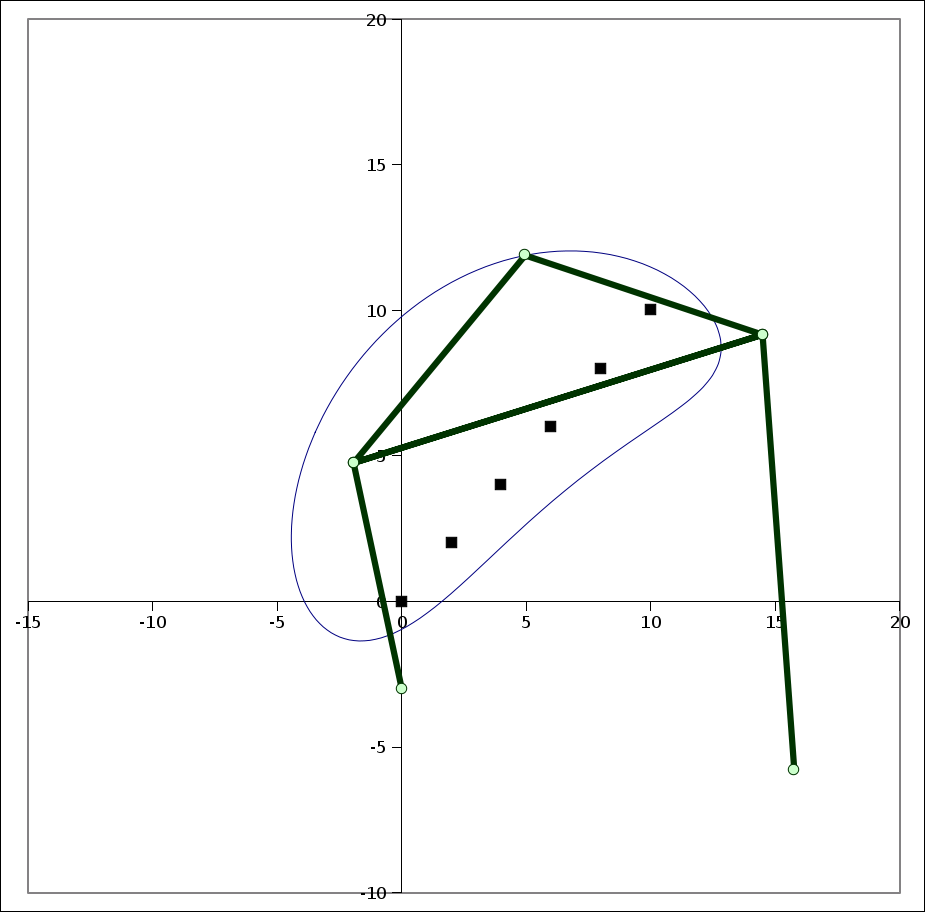
\includegraphics[width=3.0in]{apply_problem}
\label{fig:apply_problem}
\end{figure}

\begin{table}[H]
    \centering
    \caption{Nothing's Ever Good Enough, Is It?}
    \begin{tabular}{r l}
    \(r_1\): & 16\\
    \(r_2\): & 8\\
    \(r_3\): & 17\\
    \(r_4\): & 15\\
    \(\theta_1\): & \(-10^0\)\\
    \(h_x\): & 0.5\\
    \(h_y\): & 0.3\\
    \(O_x\): & 0\\
    \(O_y\): & -3
    \end{tabular}
    \label{tab:startingv}
\end{table}

\begin{table}[H]
    \centering
    \caption{I'm Pretty Sure The Spacing Is Just Coincidence.}
    \begin{tabular}{r l l}
    x & y & \(\theta_2\) \\ \hline
    0 & 0 & \(-60^0\)\\
    2 & 2 & \(-45^0\)\\
    4 & 4 & \(-30^0\)\\
    6 & 6 & \(-15^0\)\\
    8 & 8 & \(0^0\)\\
    10 & 10 & \(15^0\)
    \end{tabular}
    \label{tab:startingthetas}
\end{table}

Perhaps unsurprisingly, the software did its job, as can be seen in Figure \ref{fig:apply_solution}. 

\begin{figure}[H]
\centering
\caption{It's Like Seeing Your Baby Become An Adult.}
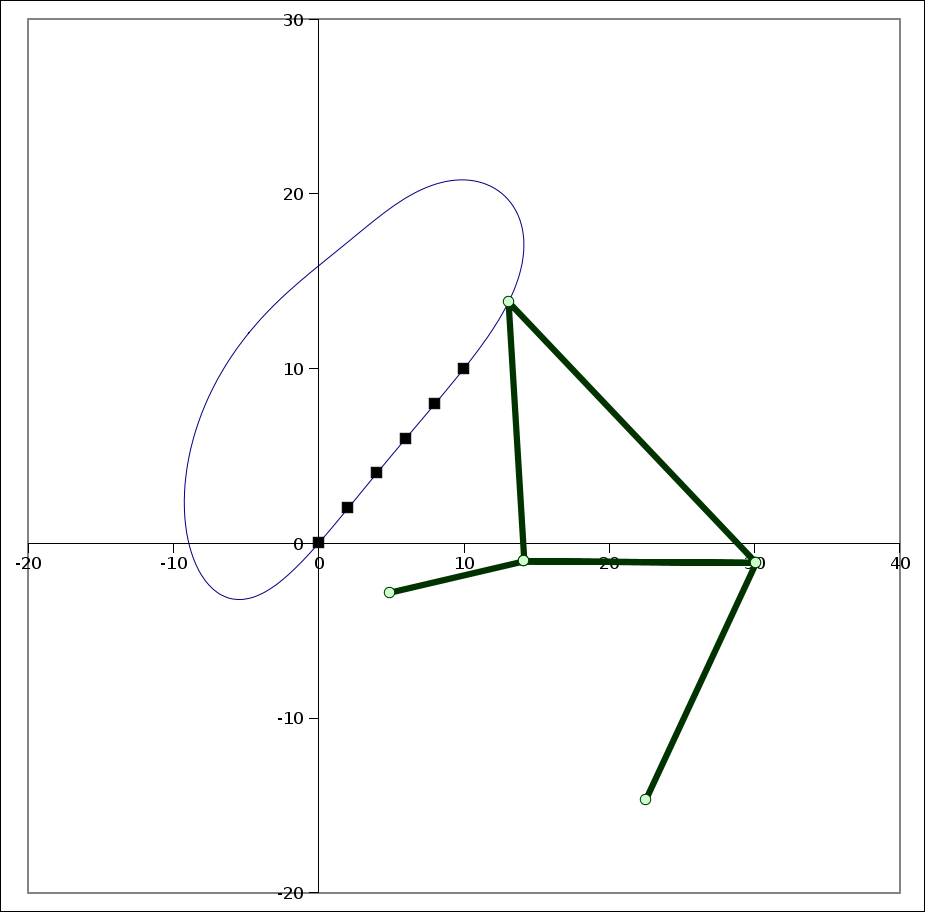
\includegraphics[width=3.0in]{apply_solution}
\label{fig:apply_solution}
\end{figure}

Perhaps disappointing is that it wasn't the same as one of the straight line linkages I saw in my kinematics textbook, but beggars can't be choosers, as it's said. 

\section*{What's Next?}

One of the major problems holding this method back (as far as I can tell) is the fact that the problem (in fact) should be constrained. Not only can the angles in \((\theta_2)_j\) fall outside the limit angle positions, but it's also possible to choose link lengths that are impossible to assemble together regardless of angles.

This has already been seen in the limitations on \(\alpha_k\) and the modification to the backtracking part of the algorithm. This protects against leaving the feasible region if the solution is feasible but \(p_k\) is extra-long. However, this does little to deal with the possible issue of there being a solution on the boundary of the feasible region.

A way to adapt to this that I considered early on was adding a penalty function to the objective function, and then adjusting the forward equations so that they return the results for the closest parameters (by some measure) in the feasible region. One problem with this, aside from the mixed performance of penalty functions, is that I didn't find this to be a huge problem in practice.

Instead, I found that it's important to have a quality starting point.  This algorithm won't converge to a single solution regardless of starting linkage--in fact, the failed benchmark was of a linkage in the same general family (crank-rockers) as the desired linkage, and it still didn't converge.

As it stands, the best way to get an initial starting point--nay, the only way--is to find one by hand, which means that there's still an element of the trial-and-error method, but with the final, more tedious refinements being done by machine.  There might be a way to generate starting linkages, but I'm not personally aware of them.

Really, what this project could use is some interface design.  In its current state, I have a spreadsheet and a set of programs that run on the command line, with the operator (me) having to copy and paste between them, converting degrees to radians and back during the process. It's certainly not how one would want to do this if he were to use this software in practice. A graphical front-end and forward linkage plotter for the curve fitting software, or even some integration between the two, would be wonderful from a usability standpoint.  One nice thing about Gnumeric is that it's extensible using python, so the latter would be relatively easy.

I also believe that there are a number of optimizations that could be made to my algorithm. For example, I don't know the best method to use for solving for the Gauss-Newton direction.  I'm currently using the conjugate gradient method to solve it, since the Jacobian (and, by extension, \(J^TJ\)) has a significant number of zero entries, but other than that I don't have a good reason for believing this to be the best method to use. In fact, it may be a particularly crummy method to use if the Jacobian tends to have poorly-scaled eigenvalues. This is just the tip of the figurative iceberg when it comes to potential and (actual) numerical waste in my algorithm.

This algorithm could also be augmented to fit against other design criteria for a linkage besides path generation. For example, one may want the path generator to travel through these points at a particular speed or acceleration, or they may want the transmission angles at these points to fit certain criteria.  Certainly, this approach could be extended to take these variables into account.

Finally, I only tested this algorithm against a few examples, all of them being 
crank-rocker linkages and all (save one) tracing simple loops instead of figure-eights or any of the other possibilities. Knowing how this algorithm behaves in more varied situations may be worth investigation.

As far as actually meeting the goals of this project, the current incarnation satisfies them nicely. Not only does the algorithm work for artificially-constructed problems designed for success, but it also works on problems where the starting point is further removed from (but ``reasonably close'' to) the solution. As this prototype demonstrates, even with all the possible complications, this sort of approach shows promise.

\end{document}

